\chapter{Framework}
\label{chap:framework}

\minitoc \mtcskip \noindent

In this chapter it is described the details and specificities of the framework proposed in this dissertation. First, we enunciate the necessary requirements to fulfill and achieve the mentioned development. Moreover, it is present the framework architecture design, as well as it inner pipeline. The modules that constitutes such architecture are described afterwards as so the required methodologies and algorithms incorporated in each of its tasks. Finally but not least, we mentioned and explained the different data visualizations available in the framework.

\section{Requirements}\label{sec:requirements}

The development of frameworks to the domain of \textit{smart cities} and intelligent transportation systems using human-generated content (e.g. text messages) is a laborious and time-consuming process. The source of the data to fed such system is one of the biggest challenges in this kind of developments, ranging from social media, smart phones and urban sensors. In this dissertation we tackle the problem of exploring social media data since this kind of data have, recently, been seen as a new opportunity and source to mine valuable information to the cities services and corresponding responsible entities~\cite{musto2015crowdpulse}.

Social media data is mostly represented by text messages being necessary the application of \gls{NLP} methodologies in order to extract information from its content. Such methodologies are usually complex and composed by several different steps (e.g. some related to the syntax of the sentences while others are related to the semantics of its content) before the achievement of the desired results. Social Media streams are no exception, indeed, the analysis of such texts is even more complex since messages are usually short and present lots of informal characteristics.

A framework for the domain of social media content requires, in the first place, a data collection module. Depending on the social network, the data collection module can have different heuristics with respect to the data retrieving. Here, the choice of such heuristics is important and needs to be made according the final users expectations, or at least, according the framework final use case. Towards the application of NLP techniques, a module in charge of preprocessing tasks is required. The main purpose of this module establishes in the performance and robustness of the results obtained by the previously mentioned techniques. NLP techniques can provide different types of information, however in this dissertation the focus is on the classification of travel-related tweets and characterization of the topic associated with a tweet. Each technique is represented as an independent module whose belongs to the boundary of text analytics. This framework needs to also be capable of processing information regarding the creation date of a tweet, \textit{metadata} and geographic distribution associated to it. For the fast retrieving of this informations to the data visualization view, some aggregations need to be made. This requirement is due to one of the big data demands, the instantly availability of the results. Such demand is important for the framework end-users since it helps in the entities' decision-making process making easier and faster the improvement of its services.

The construction of this complex system requires careful planning since there are dependency between a task and the one that follows it, at least with respect to the filtering and preprocessing of data. Adaptability to different languages is considered and further addiction of new ones may be possible. For the same reason, but this time regarding new functionalities, the framework needs to follow a modular architecture allowing new text analysis layers as well as other type of data visualizations. The domain of \textit{smart cities} is vast in terms of indicators and fields that constituting it and due to that, the final architecture may be designed in a way that allows configuration about the user's field of interest if he do not desire analytics visualization from all fields.

\section{Architecture Overview}\label{sec:architecture}

The framework proposed in this dissertation is divided into six different modules: (1) collection; (2) filtering; (3) preprocessing; (4) text analytics; (5) aggregation and (6) data visualization.

The current collection module is implemented to retrieve geo-location tweets from a specific bounding-box, however if the user demands, multiple locations can be explored at the same time. Other collection heuristics are also available, such as the keyword-search and users following. Depending on the target scenario and analytics to be explored, these two heuristics will need to be added in the module. This detail was considered during implementation period and flexibility was assured into the module composition.

Filtering tasks are directly related to \texttt{locations} heuristic of the collection module. Since this framework is designed to analyse cities or specific regions/zones of it, it is necessary guarantee if a tweet is actually inside of the searching bounding-box in order to do not induce information in the analysis from places far away of the target location. If other heuristics will be implemented, the filtering module can be configured to support other filtering-specific operations.

The preprocessing module is a module that has into consideration the future task in the framework. Having this considered, we implemented a segmented pipeline allowing the user a definition of the desired tasks he wants to analyse in the text messages since different text analysis may have different operation in the preprocessing routine. Methods implemented here are carefully described in Section~\ref{sec:text_preprocessing}.

Text analytics module is composed by two different sub-modules, both of them focusing in a specific text analysis method. Travel-related classification of tweets for two different speaking languages is available since one of the final goals regarding domain-agnostic framework is its adaptability into different scenarios and the language of texts constitutes one of them. Topic Modelling sub-module is available as a text analytics method provided by the framework. We trained a model over a sample of tweets and characterize each topic generated in order instantly characterize future tweets by only being necessary passing it over the transformation process to have their topic identified.
In terms of generalization, the main module, text analytics module, was construct following adaptability and flexibility approaches to, in the future, new analysis be integrated.

By adding new functionalities, new aggregations are required in order to present the specific-task final results to the end-user. The aggregation module is structured into integrative methods facilitating future extensions or updates on it. Last but not least, aggregation results are communicated to the visualization module, where, similar to other modules, it is possible the inclusion of new data visualization charts, according to the new integrated functionalities.

\begin{figure}[htbp]
	\centering
	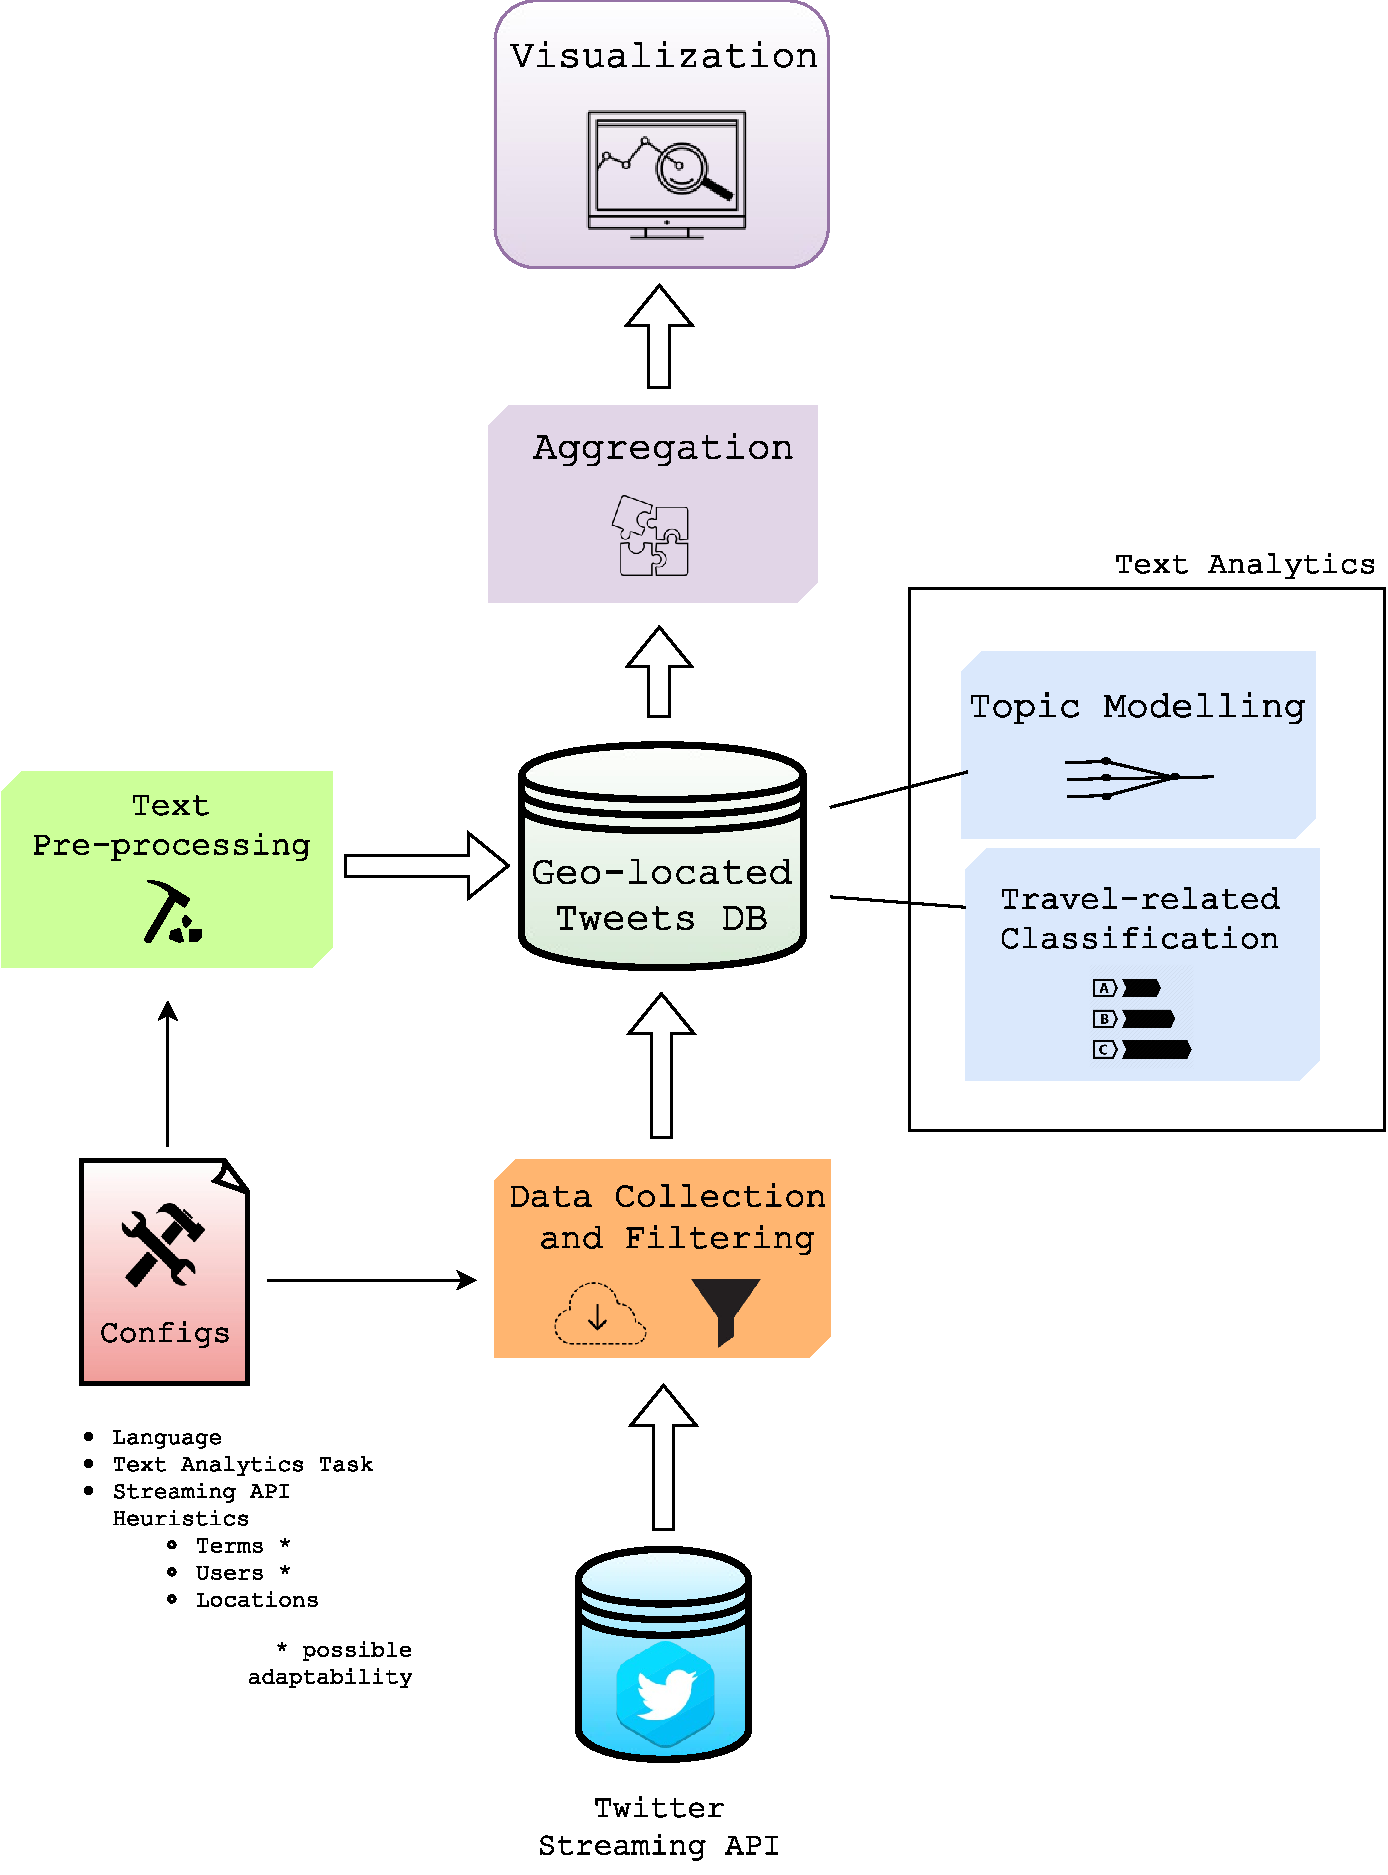
\includegraphics[width=\textwidth]{figures/architecture_2.pdf}
	\caption[Framework Architecture Overview]{Architecture overview of the implemented framework}
	\label{fig:architecture}
\end{figure}

\section{Data Collection}\label{sec:data_collection}

In Section~\ref{sec:requirements}, we explain the importance of the decision made to the data collection's heuristics. Twitter allows the developers' community two different tools to collect data, the Search and the Streaming \glspl{API}. The Search API is based on the RESTful protocol and only looks up for tweets published in the last 7 days, while the Streaming API creates basic endpoints (independent of the REST protocol) and retrieves up to 1\% of the Twitter Firehose~\footnote{Twitter Firehose - is a paid Twitter service that guarantees the delivery of 100\% of the tweets matched with certain criteria.}. Regarding the proposed and developed framework, we chose the Streaming API due to its free-access for the community, smooth integration in the module implementation and due to the availability of real-time information. A positive point about the Streaming API is the three available heuristics to the data collection, allowing the retrieval of tweets that match a specific text query (e.g. tweets with the word \texttt{bus} or \texttt{car}), the retrieval of tweets associated to a variable  number of users - being necessary previous knowledge about these users \textit{ids} - or even the retrieval of tweets located inside a bounding-box~\cite{mac2016effects}. There are two negative points regarding the Twitter Streaming API: first, Twitter imposes limits in its data exploration, where only 400 words can be tracked, 5,000 users can be followed and 25 different bounding-boxes can be explored\footnote{\url{https://dev.twitter.com/streaming/reference/post/statuses/filter} (Accessed on 18/06/2017)}; second, the previously mentioned heuristics cannot be used together, i.e. we can not track specific tweets from an user that match with certain words. Although the negative points, we remain with the choice made, of using the Twitter Streaming API as our source of information and limiting the heuristic to the one that retrieves tweets located inside a bounding-box. Our choice is additionally supported by the need of studying cities and exploring the information derived from it. This way, we know, a priori, that if the data collection method is able to retrieve tweets with precise geo-location then this makes our work easier since the exploration of specific regions of a city is already available taking into consideration the information available in tweets.

After the method selection, as well as the selection of its heuristic, we conduct an experiment regarding the amount of tweets being retrieved by one Twitter client for a city. Twitter has into consideration the number of clients used in the data collection process by tracking the IP address of the machine in the network. This constitutes a restriction to explore several cities with the same client since the Streaming API retrieves only 1\% of the total overcome. In the experiment, we tested the capacity of a client to retrieve all the tweets posted in New York City and used four different clients for it: one defined with the city bounding-box, and the other three defined with bounding-boxes of three boroughs in the city: Bronx, Brooklyn and Manhattan. Considering the bounding-boxes creation, we took support of an open-source \textit{online} tool coined BoundingBox~\footnote{\url{http://boundingbox.klokantech.com/} (Accessed on 23/06/2017)}, which is integrated with the Google Maps API and allows an user to create a bounding-box for an existing place in that API.

Results showed that the client defined with the greatest bounding-box, New York City, was able to retrieve 100\% of the tweets from the three different boroughs. This experiment is consolidated with the work of F. Morstatter et al.~\cite{morstatter2013sample} where it was compared the Streaming API's capacity, regarding geo-located tweets, against the Twitter Firehose. Authors concluded that the percentage of geo-located tweets corresponds to 1-2\% of total overcome from Twitter and the Streaming API is able to retrieve almost 90\% of it. Hence, we do not need to be concerned about how many bounding-boxes are used in the collection process because if we did so, we would need to be aware of 90\% of the world, which is not the case.

\subsection{Data Filtering}
\label{subsec:data_filtering}
In the first attempts to study the data collected geographic distribution, we discover that not all tweets had a precise coordinate attached to it. Nonetheless, there were cases where tweets from other cities were collected by our crawler and this phenomenon is not supposed to happen when the collection method is based in geo-located characteristics. By studying the Twitter mobile application, we found out that a user can tag himself in the tweet by two different ways: (1) a user can activate the GPS in the mobile application and associate to the tweet his precisely geo-location; (2) a user can choose a place from a predefined list provide by Twitter and associate the place to the tweet.

The second method of tagging the geo-location to the tweet can arise some conflicts when this kind of tweets is used to perform scientific studies or even development of system to help the cities in the regularization, control and improvement of its services. Having this considered, it was necessary to understand how the Twitter Streaming API works and what kind of heuristics follows in order to retrieve such type of tweets. The documentation~\footnote{\url{https://dev.twitter.com/streaming/overview/request-parameters\#locations} (last visited on 17 June, 2017)} enhances two different heuristics:

\begin{enumerate}
	\item If the coordinates field is populated, the values there will be tested against the bounding-box;
	\item If the coordinates field is empty but place is populated, the region defined in place is checked for intersections against the locations bounding-box. Any overlapping areas will yield a positive match.
	\end{enumerate}
	
The first heuristic only happens if a user is able/willing to tag a post with his precise geo-location associated with it; otherwise, the user can tag the post associated with a place and in this case the second heuristic is applied. Each place contained in the previous mentioned list, which is provided by Twitter, is composed by a bounding-box, and if any piece of it overlaps the bounding-box used in the collecting process, then a positive match is yielded and the tweet is retrieved. For example, if a tweet has a place such as Portugal and our filter bounding-box is defined for Porto, all tweets from place Portugal will be in our dataset, regardless the fact some tweets are posted elsewhere, such as in the city of Lisbon, very far away from Porto.

\begin{figure}[!htbp]
	\centering
	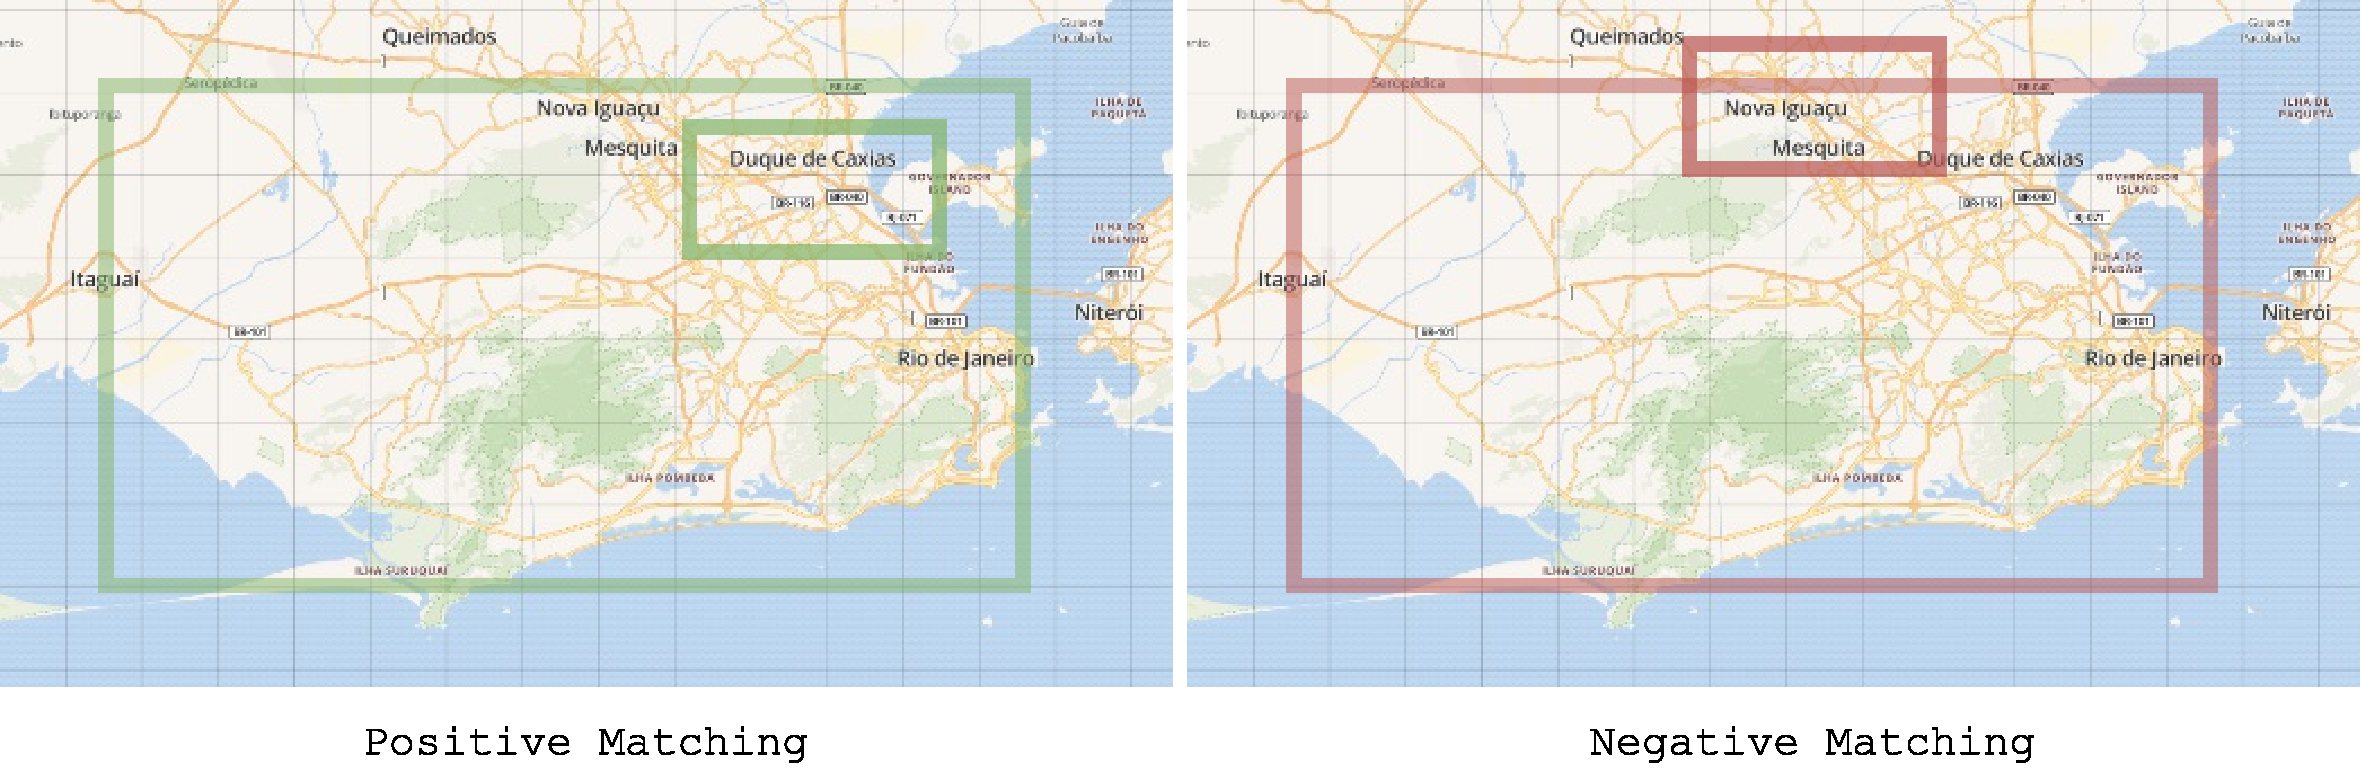
\includegraphics[width=\textwidth]{figures/bounding_boxes_matching.pdf}
	\caption{Example of our filtering method for geo-located tweets with variable bounding-boxes}
	\label{fig:matching_example}
\end{figure}

This restriction required the development of a external layer which was responsible for the filter of tweets located outside the area of each city. To built this so, it was necessary \textit{a posteriori} information and, thus, we extract the Twitter default bounding-box of each city in study appealing to the tweets \textit{place} field. Such information was then used as the limited area in order to filter out tweets which \textit{coordinates} field was not populated. The methodology behind the filtering process consists in the matching of the Twitter default bounding-box of the city against all places' bounding-boxes in tweets. In Figure~\ref{fig:matching_example}, we illustrate an example of our method in which the green color represents the matching of a tweet attached with place Duque de Caxias yielding a positive result, while the red color represents a tweet with place Nova Iguaçu yielding a negative match result with the Twitter default bounding-box for the city of Rio de Janeiro.

\section{Text Pre-processing}\label{sec:text_preprocessing}
The extraction of information from text, in particular from social media streams, is an iterative process and requires a segmented and planned pipeline to achieve the final results. In the requirements section (\ref{sec:requirements}), we mentioned some problems of social media streams as the short length and informality of the text message. The informality problem ranges from the writing style of each person to the existence of lots of abbreviations, slang, jargons, \textit{emoticons} and bad usage of punctuation signs. The preprocessing module presented in this section has as main goal the submission of the text messages under several operations in order to remove, or at least, reduce this type of informality characteristics and make easier the work of future tasks.

Below, we enumerate and described the different preprocessing methods implemented:

\begin{itemize}
	\item \textbf{Lowercasing:} This operation is responsible for the conversion upper case characters to lower representation. The advantages provided by this operation are centered in the analysis of words written in different ways. An representative example is \texttt{london} and \texttt{London} whose meaning is the same but due to the different casing in one letter, its representation/interpretation by text mining techniques may be disparate.
	
	\textit{\textbf{Travel-related Classification}} and \textit{\textbf{Topic Modelling}} modules explore this pre-processing operation.
	
	\item \textbf{Lemmatization:} Only plural words are transformed into singular ones (e.g. cars -> car).
	
	\textit{\textbf{Topic Modelling}} module explores this pre-processing operation.
	
	\item \textbf{Tokenization:} Is the method of dividing each sentence in a list of tokens/words.
	Since we are dealing with social media content, standard tokenizations techniques available in packages, such as the \texttt{tokenize}~\footnote{\url{http://www.nltk.org/api/nltk.tokenize.html}} from Python's \gls{NLTK}, perform poorly and are not capable of dealing with \textit{\#hashtags}, \textit{@mentions}, abbreviations, strings of punctuation (e.g. \texttt{...} or \texttt{\%\&\/\$}), \textit{emoticons} (e.g. \texttt{:)} or \texttt{:-)} or \texttt{=D}) and \texttt{unicode} glyphs which are very common in Twitter. Having considered this, we used a Twitter-based tokenization package, coined Twokenize and firstly presented by O'Connor et al.~\cite{o2010tweetmotif}, which is capable of dealing with these special characteristics of tweets.
	
	\textit{\textbf{Topic Modelling}} module explores this pre-processing operation.
	
	\item \textbf{Transforming repeated characters:} Sequences of characters repeated more than three times were transformed, e.g. "loooool" was converted to "loool".
	
	\textit{\textbf{Travel-related Classification}} and \textit{\textbf{Topic Modelling}} modules explore this pre-processing operation.
	
	\item \textbf{Punctuation removal:} Every punctuation symbols are removed from the text message, including the previous mentioned \textit{emoticons}.
	
	\textit{\textbf{Topic Modelling}} module explores this pre-processing operation.
	
	\item \textbf{Cleaning \textit{Entities} and Numerical Symbols:} Removing \textit{URLs}, user mentions, \textit{hashtags} and digits from the text messages.
	
	\textit{\textbf{Travel-related Classification}} and \textit{\textbf{Topic Modelling}} modules explore this pre-processing operation.
	
	\item \textbf{Stop and short words removal:} This operation consists in the removing of the most common words in the language in analysis. We used the standard words of the \gls{NLTK} Corpus package for the stop words removal task. Other type of words, such as 'kkk' or 'aff' represent short words that do not bring any valuable information from the message analysis. For this reason, we conceive a short dictionary containing these words and removed it from the message.
	
	\textit{\textbf{Travel-related Classification}} and \textit{\textbf{Topic Modelling}} modules explore this pre-processing operation.
\end{itemize}

Regarding other fields in a tweet, this module was also in charge of convert the date of creation of a tweet to the city timezone. The field \textit{created\_at} in a tweet is given in the \gls{UTC} and in order to have knowledge about the most active local hours and days on Twitter, we used the Python timezone package \texttt{pytz}~\footnote{\url{https://pypi.python.org/pypi/pytz}} to convert the world timezone to the one desired.

Although the existence of more text preprocessing techniques, in this dissertation we only used the ones previously described since each of them is associated to, at least, one text analytics module whose are described in the following section.

\section{Text Analytics}
The extraction of information from texts can vary in several types depending on the task performed to achieve it. In this dissertation, we explored two different types of analysis to the tweets: topic modelling and travel-related classification.

\subsection{Topic Modelling}
\label{sec:topic_modelling}

Further developments towards the enrichment of different information provided by the framework took us to the path of topic modelling techniques for text messages. Topic modelling is a text mining technique which goal is the identification of latent topics in a collection of documents. During the last decade, the research community had been using this technique in a vast range of works aiming the test of its applicability in different domains. Here, we also used topic modelling to characterize different cities and provide this type of information to the framework's end-users.

Latent Dirichlet Allocation (\gls{LDA}) is a generative statistical model proposed by D. Blei et al.~\cite{blei2003latent} that makes possible the discovering of unknown groups and its similarities over a collection of text documents. The model tries to identify what topics are present in a document by observing all the words that composing it, producing as final result a topic distribution. 

\begin{figure}[htbp]
	\centering
	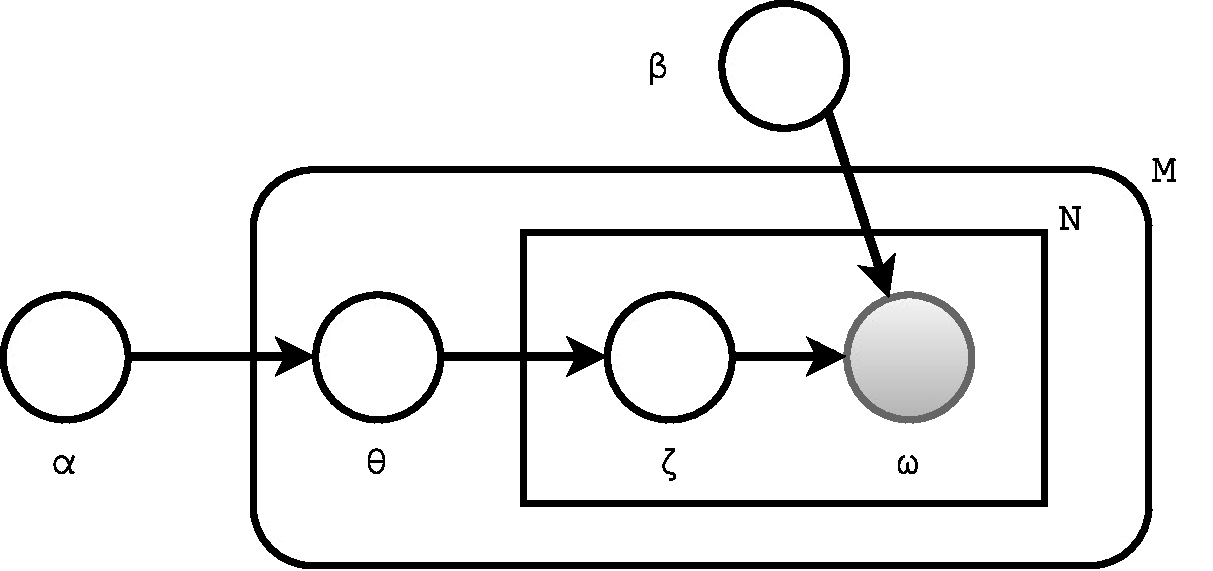
\includegraphics[scale=0.41, keepaspectratio]{figures/lda-model.pdf}
	\caption[Plate notation of \gls{LDA} by Blei et al. ~\cite{blei2003latent}]{Plate Notation of the graphical model representation of Latent Dirichlet Allocation by Blei et al. Source:~\cite{blei2003latent}}
	\label{fig:lda_graphical_model_representation}
\end{figure}

In Figure~\ref{fig:lda_graphical_model_representation} it is illustrated the plate notation to the graphical model of \gls{LDA}. There, we can observe that for a collection of documents $M$, each one composed by a sequence of $N$ words, the model tries to attribute a per-document topic distribution, using an $\alpha$ dirichlet prior, to a topic-word distribution $\xi$ (associated also with a dirichlet prior $\beta$), inducing that each topic's probability $\theta$ is focused in a small set of words $w$ which characterize that topic.

The most important advantage this model provides is related to the group of features involved in its training process. Conventional application of this model uses only as features a bag-of-words matrix representation, and for this reason the task of topic modelling becomes very simple since only the frequency of words in documents are taken into account. Last but not least, \gls{LDA} model performs two different distributions: (1) distribution of words over topics and (2) distribution of topics over the documents, resulting in the assumption that each document is random mixture of topics, whose in turn are composed by a probabilistic distribution of words.

The cities' characterization provided by our framework centers in the topics being talked about at the time. We conduct an experiment to evaluate if such information could bring added-value for the cities entities and the results although being very promiscuous proved to have potential in certain occasions. The overall experiment is described in Section~\ref{sec:topic_modeling} as well as potential improvements to the generated model.

\subsubsection{Features}
Topic modelling requires, like in other learning model, a group of features to be trained. In this case, we used the \glossary{BoW} representation matrix - which is a representation where each document is converted to a frequency vector according to the number of occurrences of each word in the message. The set of features was limit to a dictionary containing 10,000 words and it only took into account uni-grams in the message content. The dictionary was also limited to words that occur in a maximum percentage of 40$\%$ in the whole dataset, avoiding common words that were not removed because they were not included in the NLTK Stop Words list. The minimal occurrence value for a word being considered was set to 10.

\subsubsection{LDA Model Resulting Topics}
The final model used in the implementation of our framework is defined to characterize a tweet into 50 different topics. Although that, in the experiment made to comprove the added-value brought by the model,  we were obligated to cluster some of the topics due to the similarity presented in words constituting them. The final list of possible topics can be seen in Section~\ref{subsec:lda_results}, more specifically in Table~\ref{tab:final_classification}.

\subsection{Travel-related Classification}
\label{sec:travel_classification}

\emph{Prima facie}, we tried to extract and characterize travel-related tweets from large datasets in order to study the geographical and temporal distributions of such specific content. To be successful in this task it was created an automatic text classifier capable of discriminating travel-related tweets from non-related ones. Due to the absence of gold standard datasets in this domain, there was the need of creating a training and testing set of data in order to proceed the experiment and evaluate the performance of the produced model. Conventional classification tasks in the domain of intelligent transportation systems follow traditional approaches by constructing their group of features using standard bag-of-words techniques. In our experiment, we tried to combine a \gls{BoW} features with \gls{BoE} (word embeddings representation matrices), producing, for the best of our knowledge, the first travel-related classification model with both type of features.

\subsubsection{Features}
\label{sec:travel_features}
\gls{BoW} representation matrix is a list of lists, where each entry of the matrix is associated to a sentence of the document and takes the form of a term-frequency vector. In this group of features, we only considered uni-grams as the basis of text representation form. The final dictionary of this form was produced with the 3,000 most frequent terms across the training set excluding the ones found in more than 60$\%$ of the documents (tweets).

The technique of word embeddings is used by Mikolov et al.~\cite{mikolov2013efficient} in the implementation of a powerful computational method named \emph{word2vec}. This method is capable of learning distributed representations of words, and each word is represented by a distribution of weights across a fixed number of dimensions. Authors have also proved that such representation is robust when encoding syntactic and semantic similarities in the embedding space.

The training objective of the skip-gram model, as defined by Mikolov~et~al.~\cite{mikolov2013linguistic}, is to learn the target word representation, maximizing the prediction of its surrounding words given a predefined context window. For instance, to the word $w_t$, present in a vocabulary, the objective is to maximize the average log probability:

\begin{equation}
\frac{1}{T}  \sum_{t=1}^{T}  \sum_{-c \leq j \leq  c, j \neq 0} \textnormal{log } P(w_{t+j} | w_t)
\end{equation}

where $c$ is the size of the context window, $T$ is the total number of words in the vocabulary and $w_{t+j}$ is a word in the context window of $w_t$. After training, a low dimensionality embedding matrix $\textbf{E}$ encapsulates information about each word in the vocabulary and its use (i.e. the surrounding contexts). For instance, by using the skip-gram model over our datasets we were able to verify that words such as \texttt{ônibus} and \texttt{busão} are used in the similar contexts, as a mode of transport.

Later on, Le and Mikolov~\cite{le2014distributed} developed paragraph2vec, an unsupervised learning algorithm operating on pieces of text not necessarily of the same length. The model is similar to \emph{word2vec} but learns distributed representations of sentences, paragraphs or even whole documents instead of words. Hence, we explored \emph{paragraph2vec} to learn the vector representations of each tweet and tried several configurations in the model hyper-parameterization.

Using \textit{paragraph2vec}~\cite{le2014distributed}, we created bag-of-embeddings in order to explore the learning distributed representations of words where each word is represented by a distribution of weights across a fixed number of dimensions. Mikolov et al.~\cite{mikolov2013linguistic} proved that this kind of text representation is robust when encoding syntactic and semantic similarities in the embedding space. The training process of our classification models involved 10 iterations over the datasets using a context window of value 2 and feature vectors of 50, 100 and 200 dimensions. Then, the corresponding embedding matrix yielded the group of features fed into our classification routine.

Both previous described methods are available in the collection of Python scripts we used in this dissertation, coined \texttt{Gensim}~\footnote{\url{https://radimrehurek.com/gensim/about.html} (Accessed on 20/06/2017)}, presented and lately improved by \v{R}eh\r{u}\v{r}ek and Sojka~\cite{rehurek2010software}.

The overall experiments regarding the travel-related classification of tweets are described and detailed in Sections~\ref{subsec:rio_de_janeiro_sao_paulo_experiment} and~\ref{subsec:new_york_city_experiment}. Concluded the experiments, we select the best classifiers for each case and used it in the implementation of the framework's travel-related modules allowing discrimination of potential new tweets related to the transportation domain.

\subsection{Final Remarks}

The previous mentioned text analytics methodologies were implemented as separate modules in the framework since each of them needs different preprocessing operations over the data. A future interesting improvement to the framework, presented in this dissertation, is the incorporation of an extra module of sentiment analysis that should work together with the two already developed, and provide additional information about the services of a smart city, including the transportation domain.

\section{Data Storage and Aggregation}\label{sec:storage_aggregations}

Besides the few percentage of geo-located tweets provided by Twitter (1-2\% of the total Firehose overcome), this data requires, in the first place, large physical space for storage and, secondly, a tool that allows the easy manipulation and quick access of data. Having considered this, we opted for the use MongoDB, an open-source cross-platform document-oriented database, as the database system for our framework. MongoDB allows the storage of JSON-like documents which is the retrieved format of tweets by the Streaming API. Since in this dissertation we developed the framework as a prototype of a system capable of extracting information related to \textit{smart cities} and transportation services, the large physical space to storage data was not a priority.

MongoDB presents, alongside the high performance, availability and scaling, an inner framework that allows the aggregation of data according to specific user-generated queries. Here, we took advantage of such a pipeline in order to produce interesting statistics regarding the processed data. Map-reduce is the processing paradigm behind the aggregating operations allowing high performance even when applied to large volumes of data, as in this particular case where it is necessary to process thousands or millions of tweets in a short period of time.

\section{Visualization}\label{sec:visualization}

One of the most laborious and time-consuming tasks in the development of this social media based framework was the selection of data visualizations to illustrate the results provided by the previous mentioned modules. Due to the amount of data being processed, the generation of data visualization using an atomic implementation is sometimes poorly in terms of response time. Hence, we needed to adopt a different approach in order to solve this non-efficient procedure.

After a long period of research, we found a solution to this problem by creating a set of routines (bash scripts) that are called periodically (hourly) to execute all type of necessary aggregations and update its corresponding data collections in the database. Then, other routine is invoked to generate all type of data visualizations and store its visual representation in HTML files. In the implementation of this module, these files - containing the data visualization - were embedded inside several view pages. \texttt{Plotly}~\footnote{\url{https://plot.ly/python/}} is a Python graphing library that has available the saving of the visualizations produced in files with HTML format. Besides that, the library offers an extensive range of graphical representations, such as basic charts (bar charts, scatter plots, etc), scientific charts (heatmaps), financial charts (time series) and maps (choropleth, bubble and line maps), which facilitates the construction and designing of dynamic dashboards. Here, we explore mostly the section of basic charts to build simple representations of the results obtained from the analytics phase and also added top lists about some metadata of the tweets, as so the overall, daily and hourly top \textit{hashtags} and uni-grams.

%\section{Summary}